\documentclass[border={-4pt -6pt -4pt -4pt}]{standalone}

\usepackage{hyperref}
\usepackage{tikz}

\usetikzlibrary{decorations.pathreplacing,
  arrows,
  calc,
  decorations.pathmorphing,
  decorations.pathreplacing,
  decorations.markings,
  fadings,
  positioning,
  shapes,
  3d
}
\usepgfmodule{oo}

\pgfdeclareradialshading{glow2}{\pgfpoint{0cm}{0cm}}{
  color(0mm)=(white);
  color(2mm)=(white);
  color(8mm)=(black);
  color(10mm)=(black)
}

\begin{tikzfadingfrompicture}[name=glow2 fading]
  \shade [shading=glow2] (0,0) circle (1);
\end{tikzfadingfrompicture}

\ifpdf
% Ensure reproducible output
\pdfinfoomitdate=1
\pdfsuppressptexinfo=-1
\pdftrailerid{}
\hypersetup{
  pdfcreator={},
  pdfproducer={}
}
\fi

\definecolor{atomorange}{rgb}{1,0.483,0}

\pgfdeclarelayer{tweezer}
\pgfsetlayers{tweezer,main}
\pgfooclass{tweezer}{
  \method tweezer() {
  }
  \method drawAtom(#1,#2,#3,#4) {
    \fill [#4,path fading=glow2 fading] (#1,#2) circle (#3);
  }
  \method drawNaAtom(#1,#2,#3) {
    \pgfoothis.drawAtom(#1,#2,#3,orange);
  }
  \method drawCsAtom(#1,#2,#3) {
    \pgfoothis.drawAtom(#1,#2,#3,blue);
  }
}
\pgfoonew \mytweezer=new tweezer()

\begin{document}
\begin{tikzpicture}
  \node at (0.0, 0) {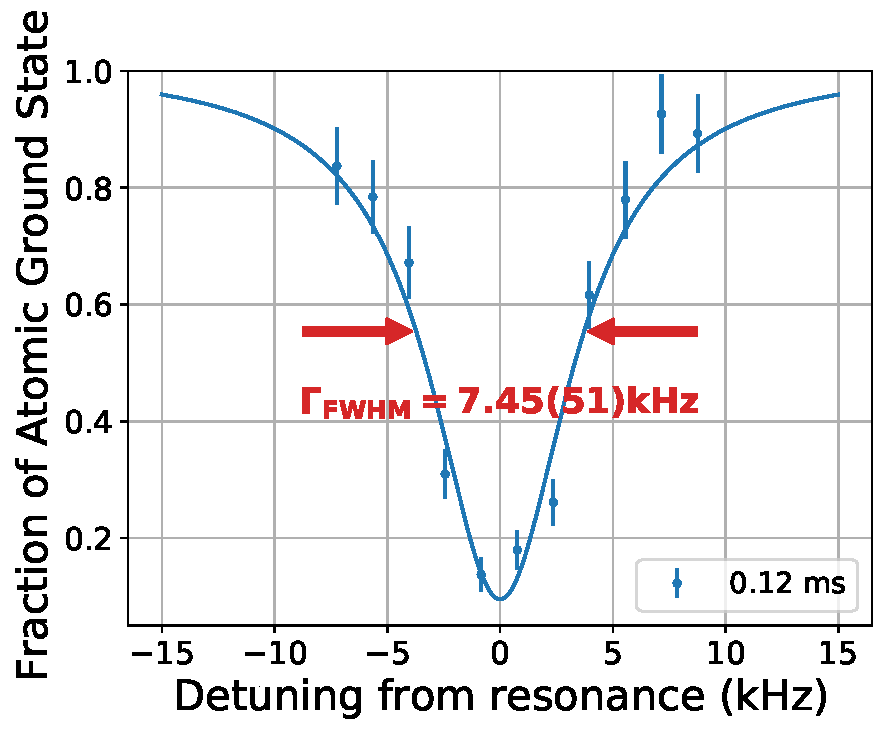
\includegraphics[height=4.586cm]{raman_transfer_fit_one_ase_freq1_fwhm.pdf}};
  \node at (-1.7, 2.0) {\scriptsize (\textbf{A})};
  \node at (5.7, 0) {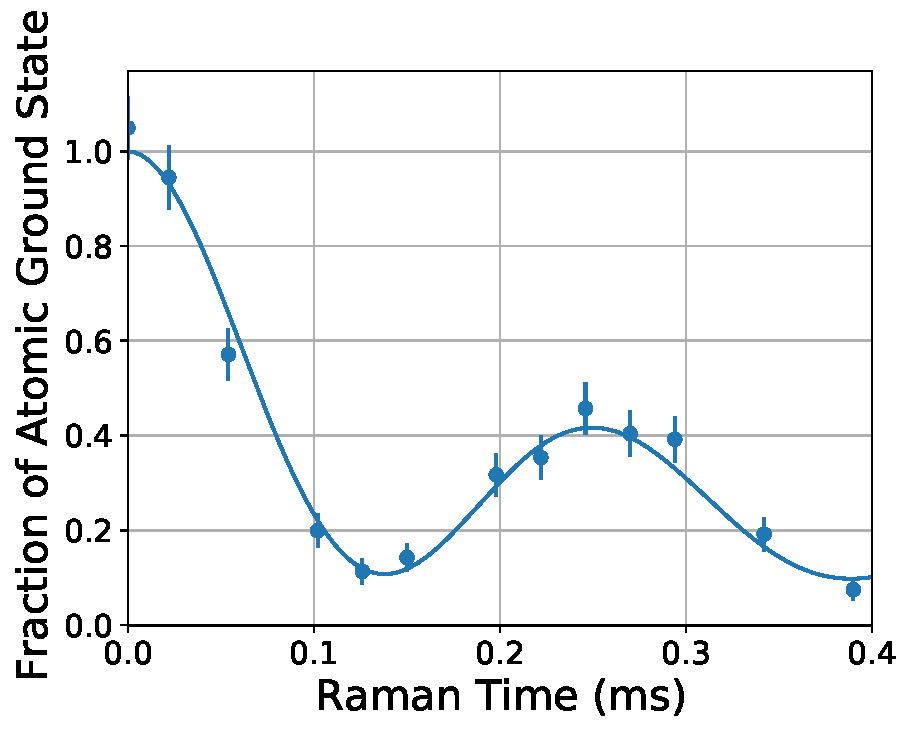
\includegraphics[height=4.586cm]{raman_transfer_fit_one_ase_time.pdf}};
  \node at (3.95, 2.0) {\scriptsize (\textbf{B})};
  \begin{scope}[shift={(4, 1.5)}]
    \draw plot[samples=200,domain=-0.2:0.2,variable=\x] ({\x + 0.06}, {\x * \x * 10 - 0.17});
    \mytweezer.drawCsAtom(0, 0.06, 0.08)
    \mytweezer.drawNaAtom(0 + 0.10, -0.05, 0.065)
  \end{scope}
  \begin{scope}[shift={(5.2, -1.5)}]
    \draw[line width=1] (0, 0.0) -- (0 + 0.15, 0.0);
    \mytweezer.drawCsAtom(0, 0, 0.08)
    \mytweezer.drawNaAtom(0 + 0.15, 0, 0.065)
  \end{scope}
  \begin{scope}[shift={(6.4, 0.1)}]
    \draw plot[samples=200,domain=-0.2:0.2,variable=\x] ({\x + 0.06}, {\x * \x * 10 - 0.17});
    \mytweezer.drawCsAtom(0, 0.06, 0.08)
    \mytweezer.drawNaAtom(0 + 0.10, -0.05, 0.065)
  \end{scope}
\end{tikzpicture}
\end{document}
